% Created 2022-09-10 sáb 18:48
% Intended LaTeX compiler: pdflatex
\documentclass[aspectratio=169, usenames,svgnames,dvipsnames]{beamer}
\usepackage[utf8]{inputenc}
\usepackage[T1]{fontenc}
\usepackage{graphicx}
\usepackage{grffile}
\usepackage{longtable}
\usepackage{wrapfig}
\usepackage{rotating}
\usepackage[normalem]{ulem}
\usepackage{amsmath}
\usepackage{textcomp}
\usepackage{amssymb}
\usepackage{capt-of}
\usepackage{hyperref}
\usepackage{color}
\usepackage{listings}
\usepackage{mathpazo}
\usepackage{gensymb}
\usepackage{amsmath}
\usepackage{diffcoeff}
\usepackage{steinmetz}
\usepackage{mathtools}
\bibliographystyle{plain}
\usepackage{siunitx}
\sisetup{output-decimal-marker={,}}
\DeclareSIUnit{\watthour}{Wh}
\hypersetup{colorlinks=true, linkcolor=Blue, urlcolor=Blue}
\renewcommand{\thefootnote}{\fnsymbol{footnote}}
\newcommand{\laplace}[1]{\mathbf{#1}(\mathbf{s})}
\newcommand{\slp}{\mathbf{s}}
\newcommand{\fasor}[1]{\mathbf{#1}(\omega)}
\newcommand{\atan}{\mathrm{atan}}
\parskip=5pt
\usetheme{Boadilla}
\usecolortheme{rose}
\usefonttheme{serif}
\author{Oscar Perpiñán Lamigueiro}
\date{}
\title{Análisis del Transitorio con la Transformada de Laplace}
\subtitle{Teoría de Circuitos III}
\setbeamercolor{alerted text}{fg=blue!50!black} \setbeamerfont{alerted text}{series=\bfseries}
\AtBeginSubsection[]{\begin{frame}[plain]\tableofcontents[currentsubsection,sectionstyle=show/shaded,subsectionstyle=show/shaded/hide]\end{frame}}
\AtBeginSection[]{\begin{frame}[plain]\tableofcontents[currentsection,hideallsubsections]\end{frame}}
\beamertemplatenavigationsymbolsempty
\setbeamertemplate{footline}[frame number]
\setbeamertemplate{itemize items}[triangle]
\setbeamertemplate{enumerate items}[circle]
\setbeamertemplate{section in toc}[circle]
\setbeamertemplate{subsection in toc}[circle]
\hypersetup{
 pdfauthor={Oscar Perpiñán Lamigueiro},
 pdftitle={Análisis del Transitorio con la Transformada de Laplace},
 pdfkeywords={},
 pdfsubject={},
 pdfcreator={Emacs 27.1 (Org mode 9.4.6)}, 
 pdflang={Spanish}}
\begin{document}

\maketitle

\section{Introducción}
\label{sec:org356ea2a}
\begin{frame}[label={sec:orga229ff0}]{Motivación}
\begin{itemize}
\item La resolución directa de las ecuaciones diferenciales (análisis clásico) exige esfuerzo y no se puede sistematizar fácilmente.
\item La transformada de Laplace convierte las ecuaciones integrodiferenciales en \alert{ecuaciones algebraicas} basadas en una variable compleja:
\end{itemize}
\[
\slp = \sigma + j\omega
\]
\begin{itemize}
\item Todos los \alert{métodos de análisis} de circuitos son \alert{aplicables} de forma directa.
\item Las \alert{condiciones iniciales} del circuito quedan incorporadas automáticamente en las ecuaciones.
\end{itemize}
\end{frame}

\section{Transformada de Laplace}
\label{sec:org06c2739}
\begin{frame}[label={sec:orgda0a503}]{Definición}
\[
  \mathcal{L}\{f(t)\} = \int_{0^-}^\infty e^{-\slp t} f(t) \mathrm{d}t = \laplace{F}
\]

\[
\slp = \sigma + j\omega
\]
\end{frame}

\begin{frame}[label={sec:org61de9b7}]{Motivación: transformada de derivadas e integrales}
\[
  \mathcal{L}\{\diff{f(t)}{t}\} =  \slp \mathbf{F}(\slp) - f(0^-)
\]

\[
  \mathcal{L}\{\diff[2]{f(t)}{t}\} = \slp^2 \laplace{F} - \slp f(0^-) - \diff*{f}{t}{0^-}
\]

\[
  \mathcal{L}\{\int_{0^-}^tf(x)\mathrm{d}t\} = \frac{\laplace{F}}{\slp} + \frac{1}{\slp} \int^{0^-}_{-\infty}f(t) \mathrm{d}t 
\]
\end{frame}


\begin{frame}[label={sec:org5d5ee07}]{Ejemplo: ecuación de un RLC serie}
\begin{block}{Ecuación diferencial}
\[
  \diff[2]{i}{t} + \frac{R}{L} \diff{i}{t} + \frac{1}{LC} i = 0
\]
\end{block}

\begin{block}{Transformada de Laplace (sin condiciones iniciales)}
\[
  \slp^2 \laplace{I} + \frac{R}{L} \slp \laplace{I}  + \frac{1}{LC} \laplace{I} = 0
\]
\end{block}

\begin{block}{Ecuación característica}
\[
  \slp^2 + \frac{R}{L} \slp  + \frac{1}{LC} = 0
\]
\end{block}
\end{frame}

\begin{frame}[label={sec:org9053afd}]{Propiedades básicas}
\begin{block}{Linealidad}
\[
\mathcal{L}\{f_1(t) + f_2(t)\} = \laplace{F_1} + \laplace{F_2}
\]

\[
\mathcal{L}\{k \cdot f(t)\} = k \cdot \laplace{F}
\]
\end{block}

\begin{block}{Desplazamiento temporal}
\[
\mathcal{L}\{f(t - \alpha)\} = e^{-\alpha \slp} \laplace{F}
\]
\end{block}

\begin{block}{Desplazamiento en frecuencia}
\[
\mathcal{L}\{e^{-\alpha t}f(t)\} = \mathbf{F}(\slp + \alpha)
\]
\end{block}
\end{frame}

\begin{frame}[label={sec:org51e323c}]{Teoremas de valor inicial y final}
\begin{itemize}
\item Útiles para comprobar una transformada o una transformada inversa.
\end{itemize}
\begin{block}{Valor inicial}
\[
f(0^+) = \lim_{\slp \to \infty} \slp \laplace{F} 
\]
\end{block}
\begin{block}{Valor final}
\[
\lim_{t \to \infty} f(t) = \lim_{\slp \to 0} \slp \laplace{F} 
\]
\end{block}
\end{frame}

\begin{frame}[label={sec:orgdd476a0}]{Transformadas importantes}
\begin{columns}
\begin{column}{0.5\columnwidth}
\[
\mathcal{L}\{u(t)\} = \frac{1}{\slp}
\]

\[
\mathcal{L}\{t\} = \frac{1}{\slp^2}
\]

\[
  \mathcal{L}\{\sin(\omega t)\} = \frac{\omega}{\slp^2 + \omega^2}
\]
\end{column}

\begin{column}{0.5\columnwidth}
\[
\mathcal{L}\{e^{-\alpha t}\} = \frac{1}{\slp + \alpha}
\]


\[
\mathcal{L}\{t^n\} = \frac{n!}{\slp^{ n+1}}
\]

\[
  \mathcal{L}\{\cos(\omega t)\} = \frac{\slp}{\slp^2 + \omega^2}
\]
\end{column}
\end{columns}
\end{frame}

\begin{frame}[label={sec:orgbb4332f}]{Transformada Inversa}
Expresamos la transformada como una fracción de polinomios:

\[
  \laplace{F} = \frac{\laplace{N}}{\laplace{D}} = K \frac{(\slp-z_1) (\slp - z_2) \ldots (\slp - z_m)}{(\slp-p_1) (\slp - p_2) \ldots (\slp - p_n)}
\]

\begin{itemize}
\item Las raíces de \(\laplace{N}\) son los \alert{ceros} de la transformada, \(z_i\).
\item Las raíces de \(\laplace{D}\) son los \alert{polos} de la transformada, \(p_i\).
\end{itemize}

\vspace{\baselineskip}

Para obtener la transformada inversa diferenciamos tres casos (o una combinación): 
\begin{itemize}
\item Polos reales únicos
\item Polos reales repetidos
\item Polos conjugados.
\end{itemize}
\end{frame}

\begin{frame}[label={sec:orgb0ac888}]{Transformada Inversa}
\begin{block}{Polos reales únicos}
Reescribimos la transformada como suma de fracciones (descomposición en fracciones parciales):
\[
  \laplace{F} = \frac{\laplace{N}}{\laplace{D}} = \frac{K_1}{\slp-p_1} + \frac{K_2}{\slp-p_2} + \ldots + \frac{K_n}{\slp-p_n} 
\]

\[
  K_i = \left[(\slp - p_i) \laplace{F}\right]_{s = p_i}
\]

\[
  f(t) = K_1 e^{p_1 t} + K_2 e^{p_2 t} + \ldots + K_n e^{p_n t}
\]
\end{block}

\begin{block}{Ejemplo 15.9 AS}
\[
  \laplace{F} = \frac{\slp^2 + 12}{\slp(\slp + 2)(\slp + 3)}
\]
\end{block}
\end{frame}


\begin{frame}[label={sec:org3e8c73b}]{Transformada Inversa}
\begin{block}{Polos reales repetidos}
Nuevamente descomposición de fracciones parciales, y calculamos coeficientes \(K_i\) con el método algebraico (véase ejemplo 15.9 de AS)
\[
  \laplace{F} = \frac{K_1}{\slp-p_1} + \frac{K_2}{(\slp-p_1)^2} + \frac{K_3}{(\slp-p_1)^3} + \ldots + \frac{K_n}{(\slp-p_1)^n} 
\]

\[
  f(t) = K_1 e^{p_1 t} + K_2 t e^{p_1 t} + K_3 t^2 e^{p_1 t} + \ldots + K_n t^{n-1} e^{p_1 t}
\]
\end{block}



\begin{block}{Ejemplo 15.10 AS}
\[
  \laplace{F} = \frac{10\slp^2 + 4}{\slp(\slp + 1)(\slp + 2)^2}
\]
\end{block}
\end{frame}


\begin{frame}[label={sec:org25b0717}]{Transformada Inversa}
\begin{block}{Polos complejos conjugados}
Nuevamente calculamos con el método algebraico, y terminamos \guillemotleft{}completando cuadrados\guillemotright{}.

\[
  \laplace{F} = \frac{\laplace{N}}{\slp^2 + a \slp + b} = \frac{A (\slp + \alpha) + B \omega}{(\slp^2 + 2\alpha \slp + \alpha^2) + \omega^2}
\]

\[
  \laplace{F} = \frac{A (\slp + \alpha)}{(\slp + \alpha)^2 + \omega^2} + \frac{B \omega}{(\slp + \alpha)^2 + \omega^2}
\]

\[
  f(t) = A e^{- \alpha t} \cos(\omega t) + B e^{- \alpha t} \sin(\omega t)
\]
\end{block}


\begin{block}{Ejemplo 15.11 AS}
\[
  \laplace{F} = \frac{20}{(\slp + 3)(\slp^2 + 8 \slp + 25)}
\]
\end{block}
\end{frame}
\section{Aplicación a Circuitos Eléctricos}
\label{sec:orgfa32570}
\begin{frame}[label={sec:orgcc6d64e}]{Resistencia}
\begin{columns}
\begin{column}{0.5\columnwidth}
\[
  v(t) = R i(t)  
\]

\[
  \laplace{U} = R \laplace{I}
\]

\[
  \mathbf{Z}_R(\slp) = R
\]
\end{column}

\begin{column}{0.5\columnwidth}
\begin{center}
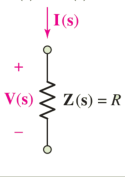
\includegraphics[height=0.8\textheight]{../figs/Resistencia_Laplace.pdf}
\end{center}
\end{column}
\end{columns}
\end{frame}

\begin{frame}[label={sec:orgb5840b2}]{Bobina}
\begin{columns}
\begin{column}{0.5\columnwidth}
\[
  v(t) = L \diff{i(t)}{t}
\]

\[
  \laplace{U} = \slp L \laplace{I} - L i(0^-)
\]

\[
  \laplace{I} = \frac{1}{\slp L} \laplace{U} + \frac{i(0^-)}{\slp}
\]

\[
  \mathbf{Z}_L(\slp) = \slp L
\]
\end{column}

\begin{column}{0.5\columnwidth}
\begin{center}
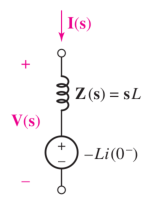
\includegraphics[height=0.4\textheight]{../figs/Bobina_Laplace_Impedancia.pdf}
\end{center}

\begin{center}
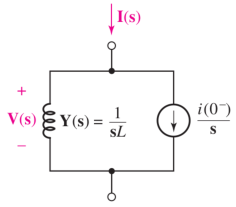
\includegraphics[height=0.4\textheight]{../figs/Bobina_Laplace_Admitancia.pdf}
\end{center}
\end{column}
\end{columns}
\end{frame}


\begin{frame}[label={sec:org3ff0315}]{Condensador}
\begin{columns}
\begin{column}{0.5\columnwidth}
\[
  i(t) = C \diff{v(t)}{t}
\]

\[
  \laplace{I} = \slp C \laplace{U} - C u(0^-)
\]

\[
  \laplace{U} = \frac{1}{\slp C} \laplace{I} + \frac{u(0^-)}{\slp}
\]

\[
  \mathbf{Z}_C(\slp) = \frac{1}{\slp C}
\]
\end{column}

\begin{column}{0.5\columnwidth}
\begin{center}
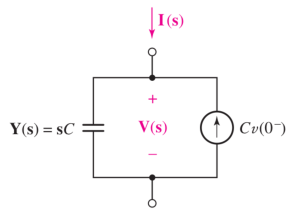
\includegraphics[height=0.4\textheight]{../figs/Condensador_Laplace_Admitancia.pdf}
\end{center}


\begin{center}
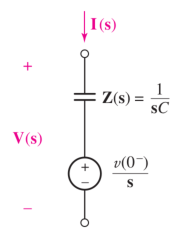
\includegraphics[height=0.4\textheight]{../figs/Condensador_Laplace_Impedancia.pdf}
\end{center}
\end{column}
\end{columns}
\end{frame}



\begin{frame}[label={sec:orgea6a0d4}]{Procedimiento}
\begin{enumerate}
\item Determinar las \alert{condiciones iniciales} en los elementos que almacenan energía: \(i_L(0^-)\), \(u_C(0^-)\).
\item \alert{Transformar} el circuito \alert{al dominio de Laplace}:
\begin{itemize}
\item Resistencia por \(\mathbf{Z}_R(\slp) = R\).
\item Bobina por \(\mathbf{Z}_L(\slp) = \slp L\) en serie con fuente de tensión de polaridad negativa.
\item Condensador por \(\mathbf{Z}_C(\slp) = \frac{1}{\slp C}\) en serie con fuente de tensión.
\item Generadores por su transformada de Laplace.
\end{itemize}
\item \alert{Resolver el circuito} con el método que corresponda (mallas, nudos, transformación de fuentes, etc.).
\item Determinar \alert{transformada inversa} de la respuesta (conviene comprobar resultado con teoremas valor inicial y final).
\end{enumerate}
\end{frame}

\begin{frame}[label={sec:orgcbd8a49}]{Ejemplo (examen 2018-19)}
\begin{columns}
\begin{column}{0.3\columnwidth}
\begin{align*}
  E_g &= \SI{500}{\volt}\\
  R_{L}&= \SI{10}{\ohm}\\
  L &= \SI{200}{\milli\henry}\\
  C &= \SI{100}{\milli\farad}\\
  R &= \SI{1}{\ohm}
\end{align*}
\end{column}

\begin{column}{0.7\columnwidth}
\begin{center}
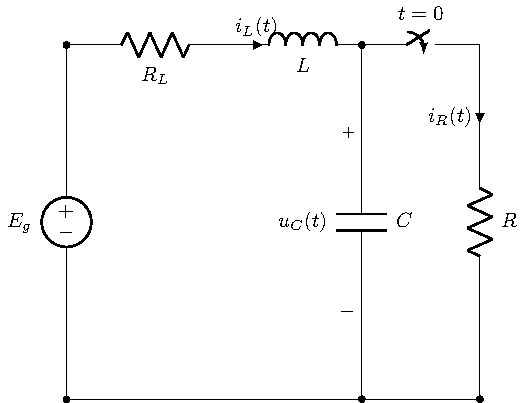
\includegraphics[width=.9\linewidth]{../figs/E2_circuito.pdf}
\end{center}
\end{column}
\end{columns}
\end{frame}

\section{Diagramas Polos y Ceros}
\label{sec:orgda63c9b}

\begin{frame}[label={sec:org76d2490}]{Función de Transferencia}
\begin{center}
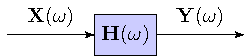
\includegraphics[height=0.2\textheight]{../figs/TransferFunction.pdf}
\end{center}

\[
  \laplace{H} = \frac{\laplace{Y}}{\laplace{X}} = K \frac{(\slp-z_1) (\slp - z_2) \ldots (\slp - z_m)}{(\slp-p_1) (\slp - p_2) \ldots (\slp - p_n)}
\]
\end{frame}


\begin{frame}[label={sec:org6d156b0}]{Polos y Ceros}
\begin{block}{Ceros}
\begin{itemize}
\item \(z_1 \ldots z_m\) son los ceros de \(\laplace{H}\)
\end{itemize}

\[
\lim_{\slp \to z_i}\laplace{H} = 0
\]

\begin{itemize}
\item Salida \(\laplace{Y}\) nula
\end{itemize}

\[
\mathbf{Y}(z_i) = \mathbf{H}(z_i) \cdot \mathbf{X}(z_i)  = 0
\]
\end{block}
\end{frame}

\begin{frame}[label={sec:orge69f9d8}]{Polos y Ceros}
\begin{block}{Polos}
\begin{itemize}
\item \(p_1 \ldots p_n\) son los polos de \(\laplace{H}\)
\end{itemize}

\[
\lim_{\slp \to p_i}\laplace{H} = \infty
\]

\begin{itemize}
\item Salida \(\laplace{Y}\) no nula para entrada \(\laplace{X}\) nula
\end{itemize}
\[
\mathbf{Y}(p_i) = \mathbf{H}(p_i) \cdot \mathbf{X}(p_i) \neq 0
\]

\begin{itemize}
\item Raíces de la ecuación característica: \alert{exponentes de la respuesta natural}
\end{itemize}

\[
  y_n(t) = \sum_{i = 1}^n A_1 e^{p_i t}
\]
\end{block}
\end{frame}

\begin{frame}[label={sec:orgede3593}]{Ejemplo Diagrama Polos y Ceros}
\begin{columns}
\begin{column}{0.3\columnwidth}
\[
\laplace{H} = \frac{\slp - \mathbf{z_1}}{(\slp - \mathbf{p_1}) \cdot (\slp - \mathbf{p_2})}
\]
\end{column}
\begin{column}{0.7\columnwidth}
\begin{center}
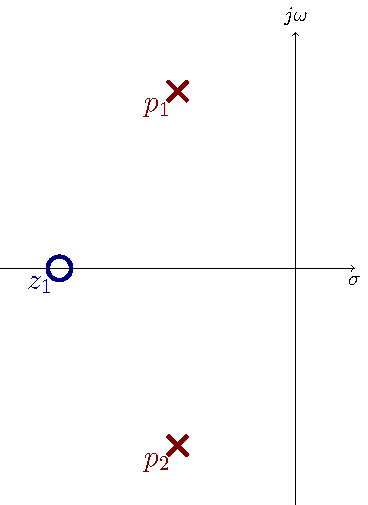
\includegraphics[height=0.7\textheight]{../figs/InterpretacionGeometrica0.pdf}
\end{center}
\end{column}
\end{columns}
\end{frame}

\begin{frame}[label={sec:org3a5f8d9}]{Significado Diagrama Polos y Ceros}
\begin{center}
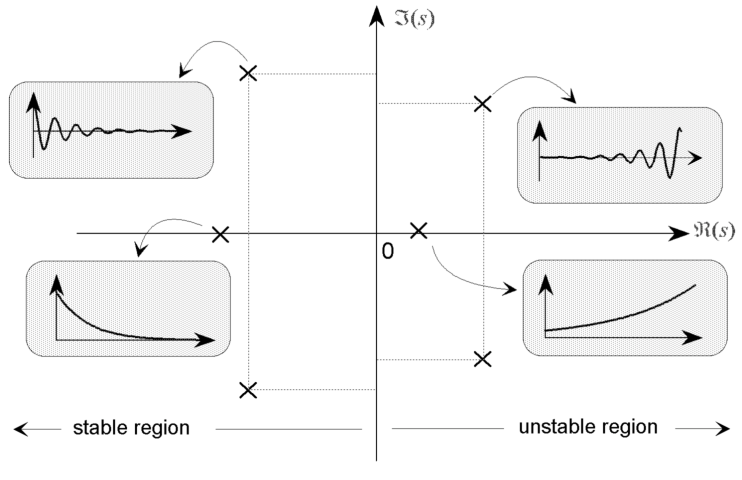
\includegraphics[height=0.8\textheight]{../figs/PoleZero.pdf}
\end{center}
\end{frame}

\begin{frame}[label={sec:orga74b492}]{Ejemplo Polos y Respuesta Natural}
\[
  y_n(t) = A_1 e^{-3t} + A_2 e^{-0.1 t} + A_3 e^{-t} \sin(2 t + \theta)
\]
\begin{center}
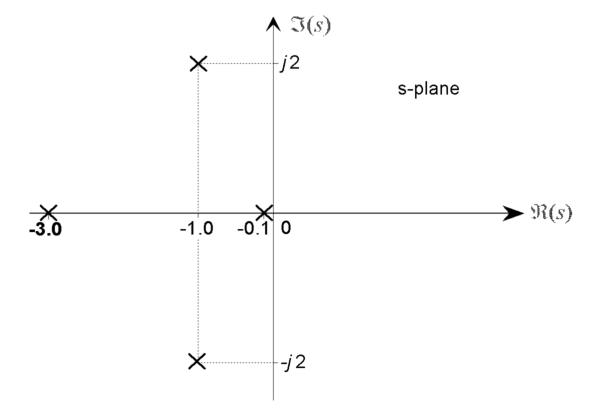
\includegraphics[height=0.8\textheight]{../figs/Ejemplo_Polos.pdf}
\end{center}
\end{frame}


\section{Ejercicios Recomendados}
\label{sec:orgade1b6c}

\begin{frame}[label={sec:orga9e1715}]{Ejercicios}
\begin{itemize}
\item AS: ejemplos 16.1, 16.3, 16.4, 16.6
\item FM: ejemplos de aplicación 4.12, 4.13, 4.14 y 4.15
\item HKD: ejemplo 15.4
\end{itemize}
\end{frame}
\end{document}